
% !TeX root = Asparsi.tex
% !BIB TS-program = biber
% !TeX encoding = UTF-8
% !TeX spellcheck = it_IT
\chapter{Triangolo}
\section{Teorema di Stewart}
\begin{thm}[Teorema di Stewart]\label{thm:Stewart}
Dato un triangolo $ABC$ colleghiamo un vertice con il lato opposto come nella figura~\cref{fig:stewart1} allora vale la relazione \[c^2y+b^2x=a(t^2+xy) \]
\end{thm}\index{Triangolo!teorema di Stewart}
\begin{figure}
	\centering
	\documentclass[10pt]{standalone}
\usepackage[utf8]{inputenc}
\usepackage{pgf,tikz,pgfplots}
\pgfplotsset{compat=1.15}
\usepackage{mathrsfs}
\usetikzlibrary{arrows}
\pagestyle{empty}
\begin{document}

\begin{tikzpicture}[line cap=round,line join=round,>=triangle 45,x=1.0cm,y=1.0cm]
\clip(0.,-0.8) rectangle (10.5,5.5);

\draw  (4.,5.)-- (10.,0.) node [midway,above] {$c$};
\draw  (10.,0.)-- (6.,0.)node [midway,below] {$y$};
\draw  (1.,0.)-- (6.,0.)node [midway,below] {$x$};
\draw  (1.,0.)-- (4.,5.)node [midway,above] {$b$};
\draw  (4.,5.)-- (6.,0.)node [midway,above] {$t$};

\draw [fill=black] (4.,5.) circle (2.0pt);
\draw[color=black] (4.14,5.33) node {$A$};
\draw [fill=black] (1.,0.) circle (2.0pt);
\draw[color=black] (0.82,-0.33) node {$B$};
\draw [fill=black] (10.,0.) circle (2.0pt);
\draw[color=black] (9.92,-0.33) node {$C$};
\draw [fill=black] (6.,0.) circle (2.0pt);
\draw[color=black] (6.02,-0.33) node {$P$};
\draw[color=black] (6.02,-0.5) node {$a$};
\end{tikzpicture}
\end{document}
	\caption{Teorema di Stewart}
	\label{fig:stewart1}
\end{figure}
\begin{proof}
Poniamo
\begin{align*}
AB=&c&&AC=b&&BC=a\\
AP=&t&&BP=x&&PC=y
\end{align*}
Indichiamo con $\alpha$ l'angolo $A\hat{P}B$ Applichiamo il teorema di Carnot\index{Triangolo!Carnot} ai triangoli $APB$ e $PCA$ avremo 
\begin{align*}
c^2=&t^2+x^2-2xt\cos\alpha\\
b^2=&t^2+y^2-2ty\cos(\pi-\alpha)\\
c^2=&t^2+x^2-2xt\cos\alpha\\
b^2=&t^2+y^2+2ty\cos\alpha\\
\intertext{Moltiplichiamo la prima per $y$ e la seconda per $x$ ottengo}
c^2y=&t^2y+x^2y-2xyt\cos\alpha\\
b^2x=&t^2x+y^2x+2xyt\cos\alpha\\
\intertext{sommando otteniamo}
c^2y+b^2x=&t^2y+x^2y+t^2x+y^2x\\
c^2y+b^2x=&t^2(x+y)+xy(x+y)\\
c^2y+b^2x=&(x+y)(t^2+xy)\\
c^2y+b^2x=&a(t^2+xy)\\
\end{align*}
come si voleva dimostrare
\end{proof}

\section{Circocentro}
\begin{defn}[Circonferenza circoscritta]\label{defn:CircCirc1}
Dato un triangolo, una circonferenza circoscritta è una circonferenza che passa per i vertici del triangolo\index{Triangolo!circonferenza!circoscritta}\index{Circonferenza!circoscritta}
\end{defn}
\begin{figure}
	\centering
\includestandalone{geometria/circumcerchio}
	\caption{Circonferenza circonscritta}
	\label{fig:circumcerchio}
\end{figure}
\begin{defn}[Circocentro]\label{defn:Circocentro1}
Il circocentro è il centro della circonferenza circonscritta. \index{Triangolo!circocentro}
\end{defn}
\begin{thm}[Assi dei lati e circocentro]\label{thm:CircoAsse1}
Il circocentro è il punto di incontro degli assi del segmento.\index{Triangolo!circocentro}\index{Triangolo!asse!lato}\index{Circocentro!triangolo}
\end{thm}
\begin{proof}
	Consideriamo il triangolo $ABC$ della figura~\cref{fig:circumcerchio2}, per comodità poniamo il vertice $A$ nell'origine degli assi e il vertice $B$ sull'asse delle $x$. Determiniamo la circonferenza che passa per i tre vertici.
	\begin{align*}
	\intertext{Considero la circonferenza generica}
	x^2+y^2+ax+by+c=&0\\
	\intertext{Passaggio per $A(0,0)$ }
	c=&0\\
	\intertext{Passaggio per $B(s,0)$}
	s^2+as+c=0\\
	\intertext{Passaggio per $C(t,r)$}
	t^2+r^2+at+br+c=&0\\
	\intertext{Risolvendo il sistema otteniamo}
	\begin{cases}	
		a=-s\\
		b=-\dfrac{t^2+r^2-ts}{r}\\
		c=0
	\end{cases}&\\
	\intertext{L'equazione cercata è}
	x^2+y^2-sx-\dfrac{t^2+r^2-ts}{r}y=0\\
	\intertext{Il centro $D$ ha coordinate:}
	\begin{cases}
	x=\dfrac{s}{2}\\ \\
	y=\dfrac{t^2+r^2-ts}{2r}\\
	\end{cases}&\\
		\end{align*}
	Troviamo l'intersezione degli assi dei lati
	\begin{align*}
	\intertext{L'asse del lato $AB$ ha equazione}
	x=&\dfrac{s}{2}\\
	\intertext{Per l'asse del lato $BC$ procediamo come segue:}
	(x-s)^2+y^2=&(x-t)^2+(x-r)^2\\
	x(2t-2s)+2ry-t^2-r^2+s^2=&0\\
	y=&\dfrac{x(s-t)}{r}+\dfrac{t^{2}+r^{2}-s^{2}}{2r}
	\intertext{Risolvendo il sistema otteniamo}
	&\begin{cases}
	x=\dfrac{s}{2}\\ \\
	y=\dfrac{t^2+r^2-ts}{2r}\\
	\end{cases}
	\end{align*}
	Da cui la tesi.
\end{proof}
\begin{figure}
	\centering
	\includestandalone{geometria/circumcerchio2}
	\caption{Circocentro ed assi segmento}
	\label{fig:circumcerchio2}
\end{figure}
\begin{cor}[Triangolo rettangolo]\label{cor:CircoAsse1}
	In un triangolo rettangolo il circocentro è il punto medio dell'ipotenusa.\index{Triangolo!rettangolo!circocentro}\index{Circocentro!triangolo!rettangolo}
\end{cor}
\begin{proof}
	Dal \cref{thm:CircoAsse1} sappiamo che il circocentro ha coordinate
	\[	\begin{cases}
	x=\dfrac{s}{2}\\ \\
	y=\dfrac{t^2+r^2-ts}{2r}\\
	\end{cases}\]
	Se come nella figura~\cref{fig:circumcerchio3} il triangolo è retto in $B$ quindi le coordinate del punto $C$ diventano $C(s,n)$ e di conseguenza quelle del punto $D$ si trasformano in 	\[	\begin{cases}
	x=\dfrac{s}{2}\\ \\
	y=\dfrac{s^2+r^2-s^2}{2r}=\dfrac{r}{2}\\
	\end{cases}\]Per verificare che il punto $D$ è sull'ipotenusa\index{Triangolo!rettangolo!ipotenusa} basta trovare l'equazione di questa. Banalmente l'ipotenusa ha equazione:
	\begin{align*}
	y=&\dfrac{r}{s}x\\
	\intertext{sostiuendo le coordinate del centro $D$}
	\dfrac{r}{2}=&\dfrac{r}{2}
	\end{align*}
	Da cui la tesi.
\end{proof}
\begin{figure}
	\centering
	\includestandalone{geometria/circumcerchio3}
	\caption{Circocentro e triangolo rettangolo}
	\label{fig:circumcerchio3}
\end{figure}
\begin{cor}[Triangolo ottusangolo]\label{cor:CircoAsse2}
	In un triangolo ottusangolo il circocentro è esterno al triangolo.\index{Triangolo!ottusangolo!circocentro}\index{Circocentro!triangolo!ottusangolo}
\end{cor}
\section{Ortocentro}
\begin{defn}[Ortocentro]\label{defn:ortocentro1}
	L'ortocentro è il punto di intersezione delle altezze di un triangolo \index{Triangolo!ortocentro}\index{Ortocentro!triangolo}
\end{defn}
\begin{thm}[Ortocentro]\label{thm:ortocentro1}
	Le altezze di un triangolo passano tutte per lo stesso punto
\end{thm}
\begin{figure}
	\centering
	\documentclass[10pt]{standalone}
\usepackage[utf8]{inputenc}
\usepackage{pgf,tikz,pgfplots}
\pgfplotsset{compat=1.15}
\usepackage{mathrsfs}
\usetikzlibrary{arrows}
\pagestyle{empty}
\begin{document}

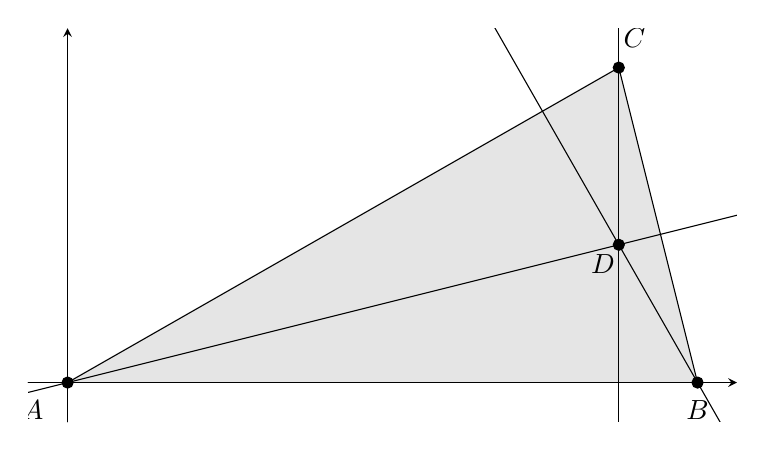
\begin{tikzpicture}[line cap=round,line join=round,>=triangle 45,x=1.0cm,y=1.0cm]
\begin{axis}[
x=1.0cm,y=1.0cm,
axis lines=middle,
ticks=none,
xmin=-0.5,
xmax=8.5,
ymin=-0.5,
ymax=4.5,]
\clip(-0.5,-0.5) rectangle (8.5,4.5);
\fill[color=black,fill=black,fill opacity=0.10000000149011612] (0.,0.) -- (7.,4.) -- (8.,0.) -- cycle;
\draw  (0.,0.)-- (7.,4.);
\draw  (7.,4.)-- (8.,0.);
\draw  (8.,0.)-- (0.,0.);
\draw  (7.,-0.5) -- (7.,4.5);
\draw [domain=-0.5:8.5] plot(\x,{(-0.--0.25*\x)/1.});
\draw [domain=-0.5:8.5] plot(\x,{(--14.-1.75*\x)/1.});
\begin{scriptsize}
\draw [fill=black] (0.,0.) circle (2.0pt);
\draw (-0.44,-0.35) node {$A$};
\draw [fill=black] (7.,4.) circle (2.0pt);
\draw (7.2,4.37) node {$C$};
\draw [fill=black] (8.,0.) circle (2.0pt);
\draw (8.0,-0.35) node {$B$};

\draw [fill=black] (7.,1.75) circle (2.0pt);
\draw[color=black] (6.8,1.5) node {$D$};
\end{scriptsize}
\end{axis}
\end{tikzpicture}
\end{document}
	\caption{Ortocentro triangolo}
	\label{fig:ortocentro1}
\end{figure}
\begin{proof}
Consideriamo un triangolo come nella figura~\cref{fig:ortocentro1}. Poniamo che $A(0,0)$, $B(0,s)$ e $C(t,r)$ otteniamo che  le altezze relative ai lati sono:
\begin{align*}
y=&-\dfrac{t}{r}(x-s)\\
x=&t\\
y=&\dfrac{s-t}{r}x\\
\intertext{mettendo a sistema le prime due otteniamo}
&\begin{cases}
y=-\dfrac{t}{r}(x-s)\\
x=t
\end{cases}\\
\intertext{otteniamo:}
&\begin{cases}
y=\dfrac{t}{r}(s-t)\\
x=t
\end{cases}\\
\intertext{mettendo a sistema le rimanenti otteniamo}
&\begin{cases}
y=\dfrac{s-t}{r}x\\
x=t
\end{cases}\\
\intertext{otteniamo:}
&\begin{cases}
y=\dfrac{t}{r}(s-t)\\
x=t
\end{cases}\\
\end{align*}
\end{proof}
\begin{cor}[Triangolo rettangolo]
Nel triangolo rettangolo l'ortocentro coincide con il vertice dell'angolo retto.
\end{cor}
\begin{proof}
Dal~\cref{thm:ortocentro1} abbiamo 
\begin{align*}
&\begin{cases}
y=\dfrac{t}{r}(s-t)\\
x=t
\end{cases}
\intertext{basta porre $s=t$ per ottenere}
&\begin{cases}
y=0\\
x=s
\end{cases}
\end{align*}
\end{proof}
\section{Triangolo equilatero}
\begin{thm}[Ortocentro e circocentro]\label{thm:triangoloequilatero1}
In un triangolo equilatero Ortocentro e Circocentro coincidono
\end{thm}\index{Triangolo!equilatero}\index{Triangolo!equilatero!ortocentro}\index{Triangolo!equilatero!circocentro}\index{Circocentro!triangolo!equilatero}\index{Ortocentro!triangolo!equilatero}
\begin{figure}
	\centering
	\documentclass[10pt]{standalone}
\usepackage[utf8]{inputenc}
\usepackage{pgf,tikz,pgfplots}
\pgfplotsset{compat=1.15}
\usepackage{mathrsfs}
\usetikzlibrary{arrows}
\pagestyle{empty}
\begin{document}

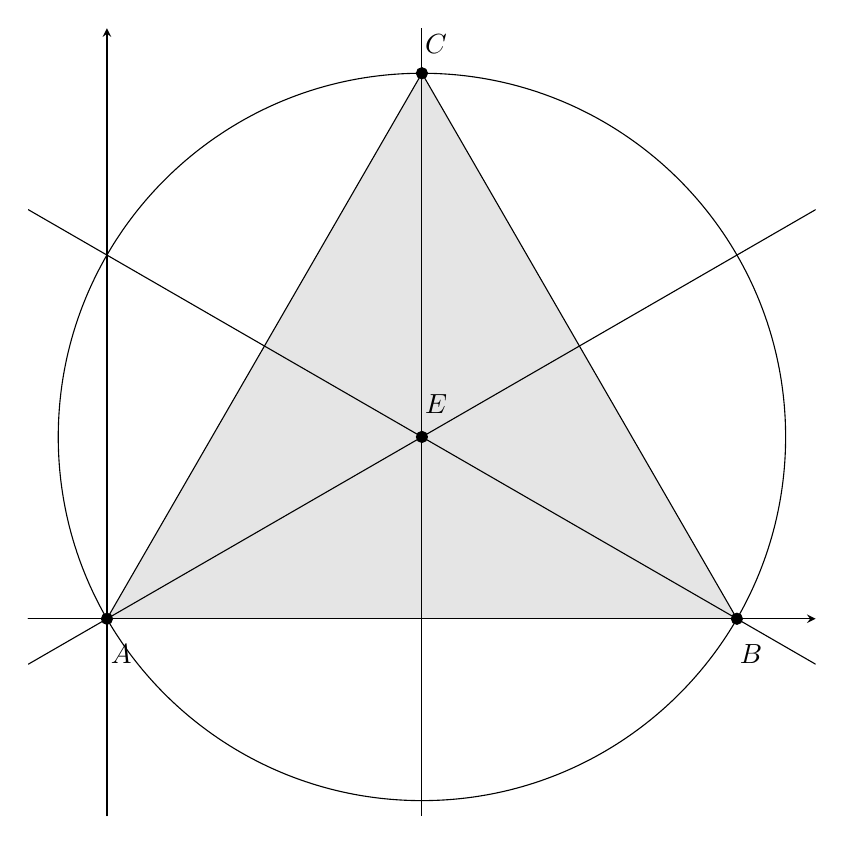
\begin{tikzpicture}[line cap=round,line join=round,>=triangle 45,x=1.0cm,y=1.0cm]
\begin{axis}[
x=1.0cm,y=1.0cm,
axis lines=middle,
%ymajorgrids=true,
%xmajorgrids=true,
xmin=-1.0,
xmax=9.0,
ymin=-2.5,
ymax=7.5,
ticks=none]
\clip(-1.,-2.5) rectangle (9.,7.5);
\fill[color=black,fill=black,fill opacity=0.1] (0.,0.) -- (8.,0.) -- (4.,6.928203230275509) -- cycle;
\draw  (0.,0.)-- (8.,0.);
\draw  (8.,0.)-- (4.,6.928203230275509);
\draw  (4.,6.928203230275509)-- (0.,0.);
\draw  (4.,2.3094010767585025) circle (4.618802153517006cm);
\draw [domain=-1.:9.] plot(\x,{(--32.-4.*\x)/6.928203230275509});
\draw [domain=-1.:9.] plot(\x,{(-0.-4.*\x)/-6.928203230275509});
\draw  (4.,-2.5) -- (4.,7.5);
\begin{scriptsize}
\draw [fill=black] (0.,0.) circle (2.0pt);
\draw (0.18,-0.45) node {$A$};
\draw [fill=black] (8.,0.) circle (2.0pt);
\draw (8.18,-0.45) node {$B$};
\draw [fill=black] (4.,6.928203230275509) circle (2.0pt);
\draw (4.18,7.3) node {$C$};

\draw [fill=black] (4.,2.3094010767585025) circle (2.0pt);
\draw (4.18,2.73) node {$E$};
\end{scriptsize}
\end{axis}
\end{tikzpicture}
\end{document}
	\caption{Triangolo equilatero}
	\label{fig:triangoloequilatero1}
\end{figure}
\begin{proof}
	Costruiamo la~\cref{fig:triangoloequilatero1}, un triangolo equilatero di lato $s$. Le coordinate del suoi vertici sono $A(0,0)$, $B(0,s)$ e $C(\frac{s}{2},\frac{s}{2}\sqrt{3})$. Per~\cref{thm:CircoAsse1} le coordinate del circocentro\index{Triangolo!circocentro}\index{Circocentro!triangolo} sono
	\[\begin{cases}
	x=\dfrac{s}{2}\\ \\
	y=\dfrac{t^2+r^2-ts}{2r}\\
	\end{cases}\]
	mentre per il~\cref{thm:ortocentro1} le coordinate dell'ortocentro\index{Triangolo!ortocentro}\index{Ortocentro!triangolo} sono \[\begin{cases}
	y=\dfrac{t}{r}(s-t)\\
	x=t
	\end{cases}\] 
	Adattando le due formule al triangolo isoscele otteniamo per entrambi:
	\[\begin{cases}
	x=\dfrac{s}{2}\\ \\
	y=\dfrac{s}{6}\sqrt{3}
	\end{cases}\]
	
\end{proof}